\documentclass[11pt]{article}
\usepackage{polski}
\usepackage[latin2]{inputenc}
\usepackage[pdftex]{graphicx}
\begin{document}
\title{Metody numeryczne. Zadanie D}
\author{Micha� Dettlaff}
\maketitle

\section{Tre�� zadania}

\noindent Napisa� program realizuj�cy metod� Eulera dla zagadnienia
\begin{displaymath} y'(t) = -y(t) - t + \int_0^t e^sy(s)ds, \end{displaymath}
\begin{displaymath}y(0) = 1 \end{displaymath}
Do aproksymacji ca�ki zastosowa� metod� trapez�w. Narysowa� wykresy rozwi�za� przybli�onych dla r�nych krok�w siatki. Rozwi�zaniem jest
$ \bar{y}(t) = \textrm{exp}(-t) $.

\section{Opis algorytmu}

Do wyznaczania kolejnych przybli�e� rozwi�zania korzystamy z wzoru:
\begin{displaymath}
  y_{n+1} = y_n + h\cdot k
\end{displaymath}
gdzie
\begin{displaymath}
  h \textrm{ - krok algorytmu}
\end{displaymath}
\begin{displaymath}
  k = f(y_n)
\end{displaymath}
W naszym przypadku wz�r b�dzie mia� posta�:
\begin{displaymath}
  y_{n+1} = y_n + h\cdot \left( -y_n(t) - t + \int_0^t e^sy_n(s)ds\right)
\end{displaymath}
Ca�k� obliczamy korzystaj�c z metody trapez�w.\newline
\begin{displaymath}
  \int_0^t e^0y_0ds =
  \frac{h}{2}y_0e^0 + \sum_{i=1}^{n-1} he^{hi} y_i + \frac{h}{2}y_ne^{hn}
\end{displaymath}
\section{Najwa�niejsze struktury programu}

{\tt F} - funkcja $ \displaystyle k = f(y_n) $\newline
{\tt INTEGRAL} - funkcja licz�ca podan� w zadaniu ca�k� metod� trapez�w\newline
{\tt y\_n } - ci�g $ \{y_n\} $

\section{Wyniki dzia�ania programu}

\noindent
B��d metody:

$$ \begin{array}[b]{lcl}
N&\vline&  \varepsilon_N\\\hline
5&\vline&  4.566\cdot10^{-2}\\
10&\vline& 2.398\cdot10^{-2}\\
20&\vline& 1.236\cdot10^{-2}\\
40&\vline& 6.290\cdot10^{-3}
\end{array} $$

\section{Wykresy rozwi�za� przybli�onych}

Dla n=5:\newline
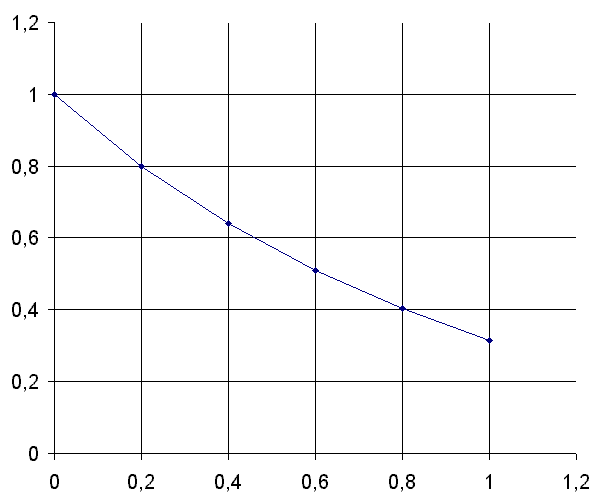
\includegraphics[scale=0.5]{n5.png}\newline
Dla n=10:\newline
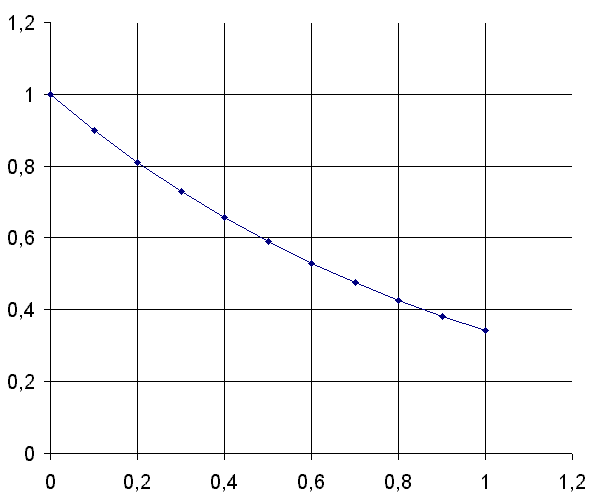
\includegraphics[scale=0.5]{n10.png}\newline
Dla n=20:\newline
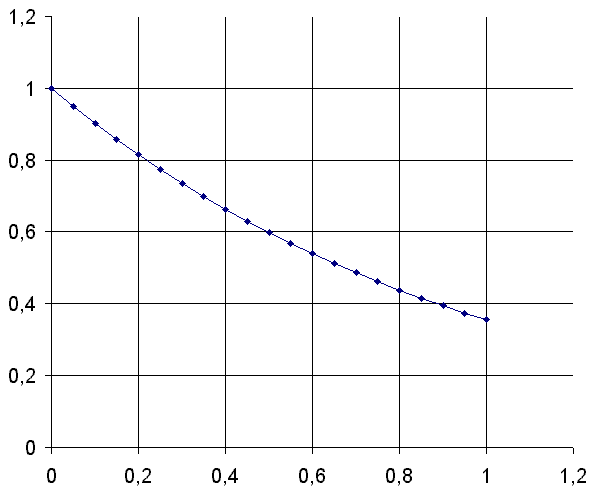
\includegraphics[scale=0.5]{n20.png}\newline
Dla n=40:\newline
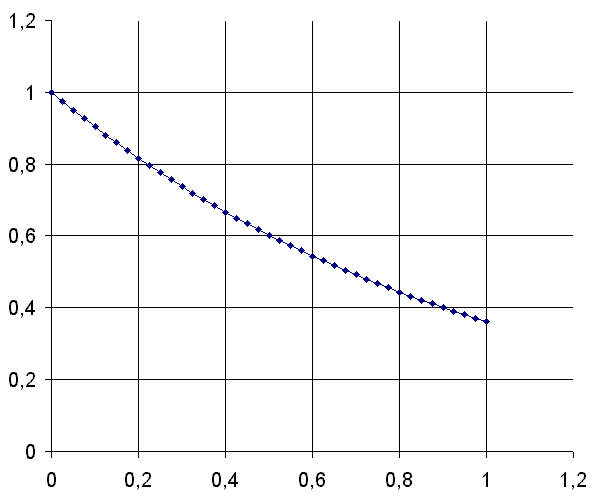
\includegraphics[scale=0.5]{n40.png}\newline

\end{document}
